\section{Classroom study setting}

 \begin{figure}
	\centering
	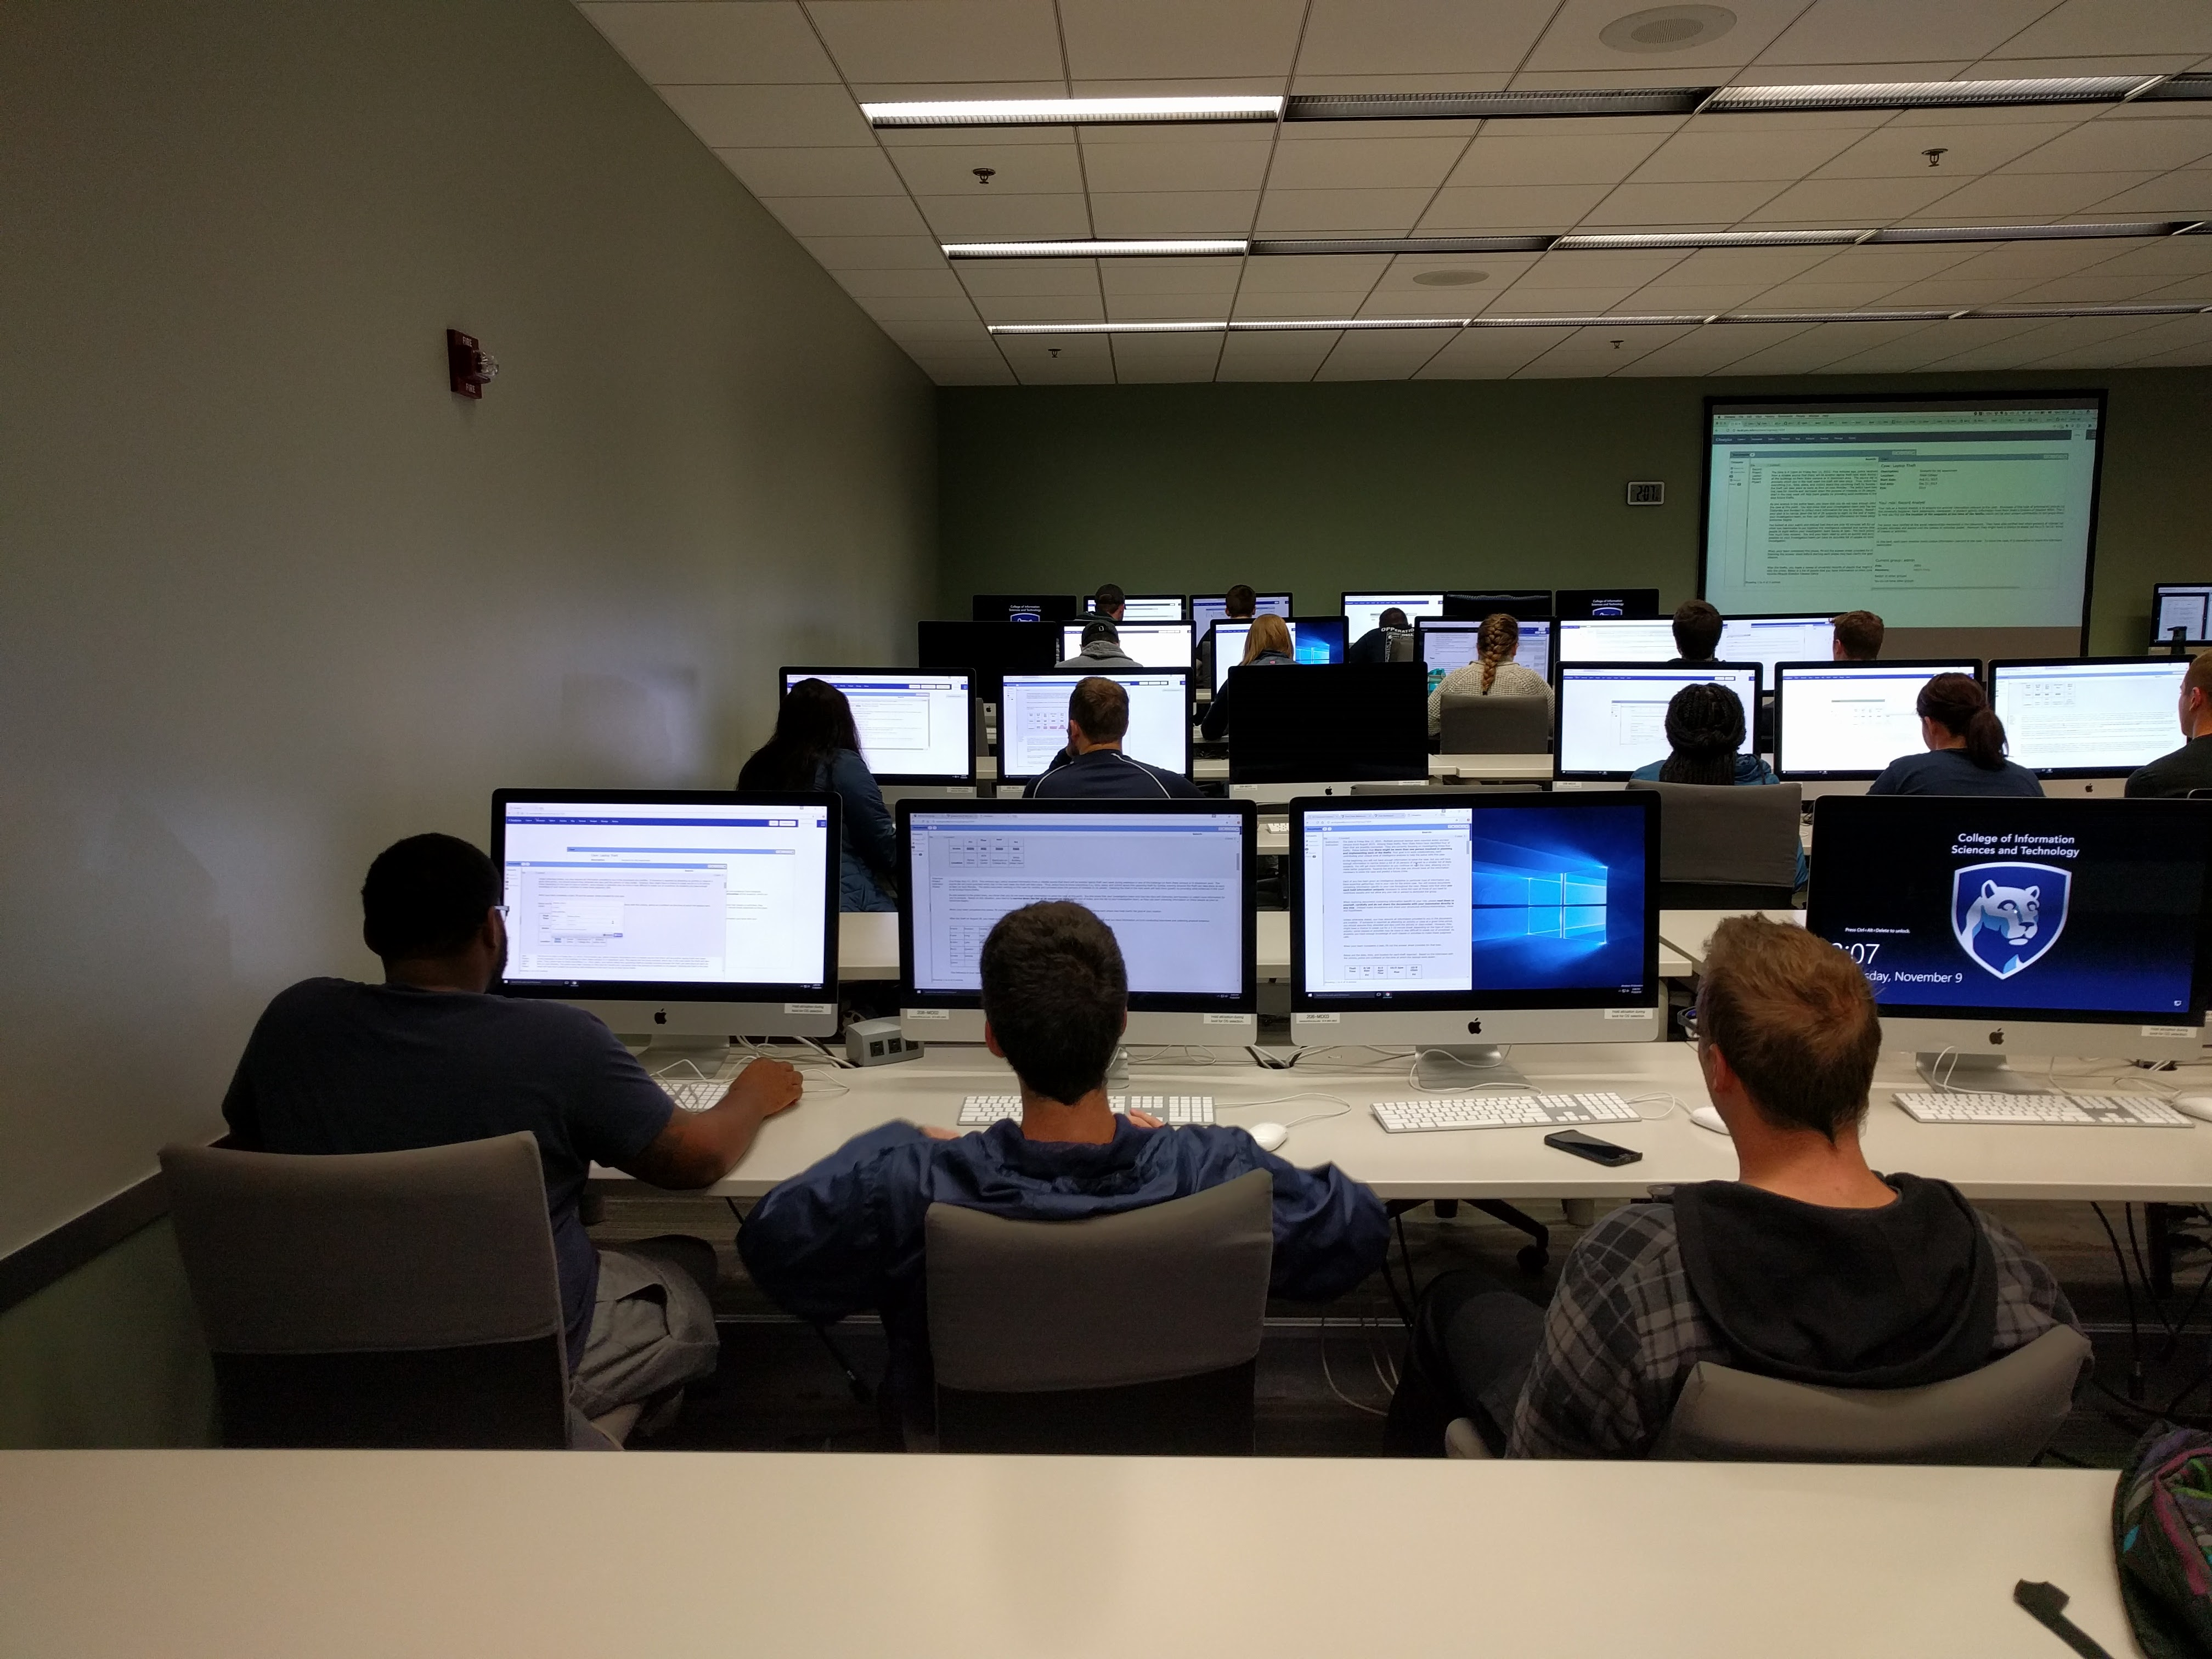
\includegraphics[width=.8\columnwidth]{05-Study_two/img/classroom_setting_2.jpg}
	\caption{The second classroom study setting}\label{fig:classroom2}
\end{figure}

We deployed CAnalytics in SRA 468, a course in the major of Security and Risk Analysis at Pennsylvania State University. The course was designed to teach senior undergraduate students about the application of visual analysis in the domain of intelligence analysis.

The study began in the later phase of the course, when students had learned about common techniques of visual analytics, such as time series analysis, tree-based data analysis, and network analysis, as well as popular visualization tools like ArcGIS and Tableau. With such equipment of basic visualization knowledge, from Nov 7 to Nov 18, we introduced CAnalytics and asked students to use the tool to solve a complex task.

Students were first given a tutorial and followed step-by-step instructions to use CAnalytics features to solve a simplified task. The students then had two full classes to do the project, each class lasting for 50 minutes. Due to the complexity of the task, students were asked to work for extra hours outside class.

The task used in the study was a fabricated laptop theft scenario. The task was applied and validated in earlier user studies \citep{Carroll2013, Borge2012}. The task consists of 222 pieces of information, involving social media data, bank transactions, suspect interviews, and other records. Teammates were randomly assigned one of the three roles and were responsible for a unique set of documents: a Web Analyst had social media data and would contribute mostly on social relationships; a Record Analyst had archival information about suspects' daily schedules and could contribute by providing locations of suspects when the theft occurred; and an Interview Analyst had interview data from people of interest and could contribute by identifying the motivation of suspects. To reach the right conclusion, teams had to share their unique information sufficiently. Students were told not to share documents directly but that they could share their information by creating data annotations in CAnalytics.

Of the 42 students enrolled in the course, 30 consented to our study and 21 (7 teams) finished the study (submitted reports for both phase 1 and phase 2 tasks). In our analysis, we focused on the 7 teams that completed both tasks. Of the 7 teams, one team (Team 163) in their post-task questionnaire reported that they ended up using Google Sheet to schematize data instead of CAnalytics. Therefore we excluded their interaction log in the analysis but kept their performance as a baseline reference for other teams.


\section{Data collection and analysis}

We did the same data collection as in the first classroom study. However, our analysis focuses on the part that relates to hypothesis development. In particular, we found user's answers to the open-ended survey questions most useful.  We asked participants to reflect the way how their team used the feature and how useful they thought of this feature. We triangulated their answer with their interaction logs captured by the system as well as hypotheses data saved in the system. This guarantees believable interpretation output in the study. In the result below, we describe our interpretations followed by users’ quoted comments. 